%%%%%%%%%%%%%%%%%%%%%%%%%%%%%%%%%%%%%%%%%%%%%%%%%%%%%%%%%%%%%%%%%%%%%%%%%%%%%
%%%%%%                                                                  %%%%% 
%%%%%%          Maqueta de memòria TFC/PFC de l'EETAC                   %%%%% 
%%%%%%                                                                  %%%%% 
%%%%%%%%%%%%%%%%%%%%%%%%%%%%%%%%%%%%%%%%%%%%%%%%%%%%%%%%%%%%%%%%%%%%%%%%%%%%%
%%%%%%%%%%%%%%%%%%%%%%%%%%%%%%%%%%%%%%%%%%%%%%%%%%%%%%%%%%%%%%%%%%%%%%%%%%%%%
%%                                                                         %%
%%          Autor: Xavier Prats i Menéndez (xavier.prats@upc.edu)          %% 
%%                  Technical University of Catalonia (UPC)                %%
%%                                                                         %%
%%%%%%%%%%%%%%%%%%%%%%%%%%%%%%%%%%%%%%%%%%%%%%%%%%%%%%%%%%%%%%%%%%%%%%%%%%%%%
%%      This work is licensed under the Creative Commons  Attribution-     %%
%%   -Noncommercial-Share Alike 3.0 Spain License. To view a copy of this  %% 
%%    license, visit http://creativecommons.org/licenses/by-nc-sa/3.0/es/  %%
%%    or send a letter to Creative Commons, 171 Second Street, Suite 300,  %%
%%                  San Francisco,California, 94105, USA.                  %%
%%%%%%%%%%%%%%%%%%%%%%%%%%%%%%%%%%%%%%%%%%%%%%%%%%%%%%%%%%%%%%%%%%%%%%%%%%%%%
%% Versió 2.1 - Juliol 2012                                                %%
%%%%%%%%%%%%%%%%%%%%%%%%%%%%%%%%%%%%%%%%%%%%%%%%%%%%%%%%%%%%%%%%%%%%%%%%%%%%%

%%% NOTA: els seguents packages son necessaris per utilitzar la
%%%       plantilla seguent:
%%%       ifthen,calc,helvet,pslatex,fancyhdr,nextpage,subfigure,tocloft,graphicx,url

%%% NOTA: Es possible que algunes distribuicions Linux o Windows.
%%%       no portin aquests paquets instal·lats per defecte.
%%%       En aquest cas els haureu d'instal·lar manualment.


%%%%%%%%%%%%%%%%%%%%%%%%%%%%%%%%%%%%%%%%%%%%%%%%%%%%%%%%%%%%%%%%%%%%%%%%%%%%%
% 1- INICIALITZACIÓ
%%%%%%%%%%%%%%%%%%%%%%%%%%%%%%%%%%%%%%%%%%%%%%%%%%%%%%%%%%%%%%%%%%%%%%%%%%%%%

\documentclass[catalan,final]{setup/eetac_tfc_pfc}
%% * OPCIONS A CONFIGURAR al \documentclass
%%    - Estat del document: final o draft
%%      NOTA: Draft no inserta les figures i marca només l'espai que
%%      ocupen. També s'indica quan el text sobrepassa els marges.
%%      Draft és molt útil per compilar ràpid el document si no és important
%%      en aquell moment visualitzar les figures.
%%    - Idioma PRINCIPAL del document: catalan, spanish, english, french...

\usepackage[english,catalan]{babel}
%%  * INCLOURE TOTS ELS IDIOMES QUE S'USARAN EN EL DOCUMENT
%%    NOTA: per canviar d'idioma al mig del document usar:
%%          \selectlanguage{nom_idioma}
%%%%%%%%%%%%%%%%%%%%%%%%%%%%%%%%%%%%%%%%%%%%%%%%%%%%%%%%%%%%%%%%%%%%%%%%%%%%%

%%%%%%%%%%%%%%%%%%%%%%%%%%%%%%%%%%%%%%%%%%%%%%%%%%%%%%%%%%%%%%%%%%%%%%%%%%%%%
% 2- CÀRREGA DE PAQUETS ADICIONALS (OPCIONALS)
%%%%%%%%%%%%%%%%%%%%%%%%%%%%%%%%%%%%%%%%%%%%%%%%%%%%%%%%%%%%%%%%%%%%%%%%%%%%%

%%% NOTA: Es possible que algunes distribuicions Linux o Windows.
%%%       no portin aquests paquets instal·lats per defecte.
%%%       En aquest cas els haureu d'instal·lar manualment.

%% El paquet inputenc és extramadament útil. 
%% Permet escriure els accents directament amb l'editor de texte
%% sense haver de fer coses com per exemple: introducci\'o
%% Heu d'especificar la codificació de caracters que utilitzeu pel
%% vostre fitxer (en aquest exemple utf8)
\usepackage[utf8]{inputenc}

%% Símbols matemàtics de la American Mathematical Society
\usepackage{amssymb,amsmath, amsfonts}  

%% El paquet array proporciona eines molt útils a l'hora de fer 
%% equacions amb matrius
\usepackage{array}             

%% Paquet que permet fer taules fusionant cel·les de files consecutives
\usepackage{multirow}          

%% Paquet molt útil en cas de tenir taules molt llargues que 
%   ocupin vàries pàgines
\usepackage{longtable}          

%% Permet canviar els colors del document
%\usepackage{color,colortbl}

%% Paquet molt útil que permet activar links en el PDF final.
%% * NO OBLIDAR DE CONFIGURAR els quatre primer camps!
\usepackage[
  pdfauthor={Nom Cognoms autor},            % Configurar adientment
  %pdftitle={Treball Fi de Carrera - autor}, % Configurar adientment
  %pdfsubject={Titol del TFC aqui},          % Configurar adientment
  % Modificació respecte a la versió 2.1 - Iván Padilla Montero - Juliol 2014
  pdftitle={Treball Fi de Grau - Sergi Garreta Serra}, % Configurar adientment
  pdfsubject={Titol del TFG aqui},          % Configurar adientment  
  pdfkeywords={keyword1, keyword2, ...},    % Configurar adientment
  pdfcreator={EETAC-UPC}, 
  pdfproducer={LaTeX, dvipdf},
  pdfdisplaydoctitle=true, plainpages=false, linktocpage=true,         
  colorlinks=true, linkcolor=blue,citecolor=blue,urlcolor=blue,
  hyperfootnotes=false, pagebackref=true, pdfpagelabels=true,
  pdfpagemode=UseOutlines,
]{hyperref} 

%% NOTA IMPORTANT!:
%% Per tal que hyperef funcioni correctament amb els capitols o seccions no
%% numerats (\chapter*{}), com per exemple introducció, conclusions i bibliografia
%% cal posar les dues comandes seguents ABANS del \chapter*{} en questió
%\cleardoublepage
%\phantomsection

%% Permet trencar links URL. 
%% Atenció! afegir aquest paquet DESPRES del hyperref!!
\usepackage{breakurl} 

%% Permet arranjar matricialment multiples figures
%% NOTA: afegir aquest paquet DESPRES del hyperref!!
%%       Si no es desitja utilitzar aquest paquet, comentar la linia seguent
%%       i anar TAMBE al fitxer de classe (eetac_tfc_pfc.cls) per substituir: 
%%       \RequirePackage[subfigure]{tocloft}  per  \RequirePackage{tocloft}
\usepackage{subfigmat}         

%%%%%%%%%%%%%%%%%%%%%%%%%%%%%%%%%%%%%%%%%%%%%%%%%%%%%%%%%%%%%%%%%%%%%%%%%%%%%


%%%%%%%%%%%%%%%%%%%%%%%%%%%%%%%%%%%%%%%%%%%%%%%%%%%%%%%%%%%%%%%%%%%%%%%%%%%%%
% 3- DOCUMENT
%%%%%%%%%%%%%%%%%%%%%%%%%%%%%%%%%%%%%%%%%%%%%%%%%%%%%%%%%%%%%%%%%%%%%%%%%%%%%

%%% Configuració de les dades i variables boleanes rellevants del document:
%%%%%%%%%%%%%%%%%%%%%%%%%%%%%%%%%%%%%%%%%%%%%%%%%%%%%%%%%%%%%%%%%%%%%%%%%%%%%
%%%%%%                                                                  %%%%% 
%%%%%%       Fitxer de dades per la memoria TFC/PFC de l'EETAC          %%%%% 
%%%%%%                                                                  %%%%% 
%%%%%%%%%%%%%%%%%%%%%%%%%%%%%%%%%%%%%%%%%%%%%%%%%%%%%%%%%%%%%%%%%%%%%%%%%%%%%
%%%%%%%%%%%%%%%%%%%%%%%%%%%%%%%%%%%%%%%%%%%%%%%%%%%%%%%%%%%%%%%%%%%%%%%%%%%%%
%%                                                                         %%
%%          Autor: Xavier Prats i Menendez (xavier.prats@upc.edu)          %% 
%%                  Technical University of Catalonia (UPC)                %%
%%                                                                         %%
%%%%%%%%%%%%%%%%%%%%%%%%%%%%%%%%%%%%%%%%%%%%%%%%%%%%%%%%%%%%%%%%%%%%%%%%%%%%%
%%      This work is licensed under the Creative Commons  Attribution-     %%
%%   -Noncommercial-Share Alike 3.0 Spain License. To view a copy of this  %% 
%%    license, visit http://creativecommons.org/licenses/by-nc-sa/3.0/es/  %%
%%    or send a letter to Creative Commons, 171 Second Street, Suite 300,  %%
%%                  San Francisco,California, 94105, USA.                  %%
%%%%%%%%%%%%%%%%%%%%%%%%%%%%%%%%%%%%%%%%%%%%%%%%%%%%%%%%%%%%%%%%%%%%%%%%%%%%%
%% Versio 2.1 - Juliol 2012                                                %%
%%%%%%%%%%%%%%%%%%%%%%%%%%%%%%%%%%%%%%%%%%%%%%%%%%%%%%%%%%%%%%%%%%%%%%%%%%%%%

%%%%%%%%%%%%%%%%%%%%%%%%%%%%%%%%%%%%%%%%%%%%%%%%%%%%%%%%%%%%%%%%%%%%%%%%%%%%%%%
%%  VARIABLES A CONFIGURAR                                                  %%%
%%%%%%%%%%%%%%%%%%%%%%%%%%%%%%%%%%%%%%%%%%%%%%%%%%%%%%%%%%%%%%%%%%%%%%%%%%%%%%%

%% - Projecte o Treball de Fi de Carrera?
%%      PFC = true   -> Projecte de Fi de Carrera
%%      PFC = false  -> Treball  de Fi de Carrera
\setboolean{PFC}{false}

%% - Escollir la titulació
%\titulacio{Enginyeria Tècnica Aeronàutica, especialitat Aeronavegació}
%\titulacio{Enginyeria T\`ecnica de Telecomunicaci\'o, especialitat Sistemes de Telecomunicaci\'o}
%\titulacio{Enginyeria T\`ecnica de Telecomunicaci\'o, especialitat Telem\`atica}
%\titulacio{Enginyeria de Telecomunicaci\'o (segon cicle)}
% Modificació respecte a la versió 2.1 - Iván Padilla Montero - Juliol 2014
%\titulacio{Grau en Enginyeria d'Aeronavegaci\'o}
%\titulacio{Grau en Enginyeria d'Aeroports}
%\titulacio{Grau en Enginyeria Telemàtica}
\titulacio{Grau en Enginyeria de Sistemes de Telecomunicació}


%% - Configurar els idiomes del document
%% Si l'idioma PRINCIPAL del document es l'angles, posar aquesta variable a true
\setboolean{Leng}{false}

%% Escollir entre catala i castella (idioma principial, o nomes pel resum en cas que l'idioma principal sigui anglès)
%%  catala = true   -> idioma principal (o només resum) en Català
%%  catala = false  -> idioma principal (o només resum) en Castella
\setboolean{Lcat}{true}

%% Titol del document en l'idioma principal del document 
\titol{Disseny d'una xarxa sense fils de sensors amb Bluetooth Low Energy per a mesures biològiques i mediambientals}

%% Titol del document en anglès (Per l'apartat overview)
\titolE{ Design of a Wireless Sensor Network (WSN) using Bluetooth Low Energy (BLE) for environmental and biological measurements for Internet of Things (IoT)}

%% Titol del document en catala/castella (Per l'apartat resum)
\titolC{Disseny d'una xarxa sense fils de sensors amb Bluetooth Low Energy per a mesures biològiques i mediambientals}


%% - Nombre d'autors del TFC/PFC?
%%      UNautor = true   Un sol autor
%%      UNautor = false  Més d'un autor
\setboolean{UNautor}{true}

%% - Nom del(s) Autor(s) del document
%% NOTA: En cas de mes d'un autor cal posar la comana \and entre els
%%        noms dels autors
\autor{Sergi Garreta Serra}

%% - Nombre de directors del TFC/PFC. Tipicament 1 o 2
%%      UNdirector = true   Un sol director
%%      UNdirector = false  Dos directors
\setboolean{UNdirector}{true}

%% - Nom del Director del TFC/PFC
\director{Josep Polo Cantero}

%% - Nom del segon director en cas de tenir-lo:
\segonDirector{Director 2}


%% - Es vol incloure una dedicatoria?
%%      dedicatoria = true   -> S'afegeix una pagina amb \textDedicatoria
%%      dedicatoria = true   -> No s'afegeix dedicatoria
%% NOTA: no confondre dedicatòria amb agraïments. Una dedicatoria sol ser
%%       un missatge curt d'una o dues frases màxim a la persona, o persones
%%       a les quals es dedica el treball. 
%%       Els agraïments poden ser extensos i l'autor pot agraïr a diverses
%%       persones coses diferents en funció de l'ajuda rebuda, per exemple. 
%%       Si es volen incloure agraïments, fer-ho al fitxer de la 
%%       memòria creant una secció nova amb  \chapter*{Agraïments}
\setboolean{dedicatoria}{true}
\textDedicatoria{A la Rocío per la seva paciència i ajuda.}

%% - Es vol incloure una pagina d'index de figures?
\setboolean{paginaLOF}{true}  % List of Figures

%% - Es vol incloure una pagina d'index de taules?
\setboolean{paginaLOT}{true}  % List of Tables 

%% - El projecte ha estat supervisat per alguna persona externa? 
%%   (NOMES en cas de practiques en empresa)
%%      supervisor = true    -> Hi ha un supervisor
%%      supervisor = false   -> No hi ha un supervisor
\setboolean{supervisor}{false}

%% NOMES en el cas de practiques en empresa (supervisor=true) s'han de 
%% configurar les variables seguents: 

%% Supervisor del TFC/PFC 
\supervisor{Nom del Supervisor}

%% - Es vol incloure el logotip de l'empresa?
%%   En el cas que el TFC/PFC s'hagi fet en règim d'intercanvi amb una
%%   empresa, es pot afegir el seu logotip a la cantonada superior
%%   dreta de la portada. En aquest cas:
%%   - posar logo=true
%%   - posar el path de la imatge i l'alçada del logo a \mylogo
\setboolean{logo}{false}
\mylogo{./setup/EETAC-positiu-negre}{1.5cm}
  

%%% Configuració de MACROS o ENTORNS (opcionals) definides per l'usuari:
\input{setup/user-macros.tex}  

%%% Configuració manual de les regles d'hyphenation:
\input{setup/hyphenation.tex}  

\begin{document}

%% Seleccionar l'idioma principal del document:
\selectlanguage{catalan}

\beforepreface  

%% RESUM i OVERVIEW
%%%%%%%%%%%%%%%%%%%%%%%%%%%%%%%%%%%%%%%%%%%%%%%%%%%%%%%%%%%%%%%%%%%%%%%%%%%%%
% NOTA: les longituds passades com a parametres d'entrada  s'han
%        d'ajustar manualment fins que el requadre del resum/overview
%        ocupi tota la pàgina. 

%%% Resum en català (o castellà)
\selectlanguage{catalan}   
\begin{resum}{10cm}
  Aquest document conté les pautes del format de presentació del treball o projecte de final de carrera. En tot cas, cal tenir en compte el que estableix la ``Normativa del treball de fi de carrera (TFC) i del projecte de fi de carrera (PFC)'' aprovada per la Comissió Permanent de l'EETAC, especialment l'apartat ``Requeriments del treball''.
\end{resum}

%%% Resum en anglès
\selectlanguage{english}   
\begin{overview}{11cm}
  This document contains guidelines for writing your TFC/PFC. However, you should also take into consideration the standards established in the document Normativa del treball de fi de carrera (TFC) i del projecte de fi de carrera (PFC), paying special attention to the section Requeriments del treball, as this document has been approved by the EETAC Standing Committee
\end{overview}

% Tornar a l'idioma principal del document
\selectlanguage{catalan}  

%NOTA: En cas d'utilitzar l'espanyol com a idioma principal del document, el
%      latex anomena les taules com a 'Cuadros'. Si es desitja canviar aquesta
%      nomenclatura i utilitzar la paraula 'Tabla' descomentar les línies següents:
%\def\listtablename{Índice de tablas}
%\def\tablename{Tabla}%



% Amb aqueta comanda indiquem que ja s'han inclòs tots els apartats del prefaci del 
% projecte o podem començar a incloure els capitols de la memòria
\afterpreface


%%%%%%%%%%%%%%%%%%%%%%%%%%%%%%%%%%%%%%%%%%%%%%%%%%%%%%%%%%%%%%%%%%%%%%%%%%
%%%%%% INCLOURE A PARTIR D'AQUÍ TOTS ELS CAPÍTOLS DE LA MEMORIA   %%%%%%%%
%%%%%%%%%%%%%%%%%%%%%%%%%%%%%%%%%%%%%%%%%%%%%%%%%%%%%%%%%%%%%%%%%%%%%%%%%%

% NOTA: recordar que la introducció i les conclusions són capítols NO
%       enumerats, per tant s'ha d'usar \chapter*

% NOTA: és aconsellable incloure els capítols de la memòria en fitxers 
%       separats utlitzant la comanda \input  Per exemple:
%       \input{capitol1}  
%       que farà que s'inclogui el fitxer capitol1.tex

% NOTA: Si es vol incloure agraïments i/o glosari, fer-ho utilitzant 
% \chapter*{} i incloure'ls abans la introducció

\cleardoublepage
\phantomsection
\chapter*{Introducció}
L'arquitectura Internet de les Coses (Internet of Things, IoT) que s'ha popularitzat en els últims anys ha comportat unes noves necessitats en molts aspectes de la tecnologia que són molt diferents dels anteriors.
Quan el que es vol és que tot estigui connectat entre si, queda clar que es trenquen moltes premisses amb les quals s'havien dissenyat originalment les tecnologies més importants que s'utilitzen avui en dia.

La transició cap a l'Internet of Things, transforma el paradigma de les comunicacions de pocs elements a molta velocitat (xarxes centralitzades) cap a molts elements amb poca velocitat (xarxes distribuïdes).
Això afecta les tecnologies sense fils que no havien estat dissenyades pel seu ús tan generalitzat.

Aquests canvis es poden veure en l'evolució de la majoria de tecnologies sense fils com wifi, xarxes cel·lulars i Bluetooth, entre d'altres.
En totes aquestes tecnologies ha estat necessari fer grans canvis per acomodar a molts més usuaris dels que s'havien predit inicialment.

El Bluetooth clàssic és un exemple d'una tecnologia que tenia limitacions a l'hora d'utilitzar-se en certs escenaris.
No permetia la comunicació entre més d'un dispositiu alhora, tenia un abast limitat i poques mesures per contrarestar les interferències.
Al llarg de la seva història, es van definir noves versions que anaven millorant les mancances del protocol.
Tot i això, el cost que suposava haver d'establir una connexió per transmetre dades, encara que fossin molt poques, seguia sent molt alt.

És per això que Bluetooth va incorporar, amb implementació opcional, l'extensió Low Energy a l'estàndard.
En aquesta extensió està definit el protocol anomenat Bluetooth Low Energy que permet molt fàcilment i utilitzant molt poca energia transmetre dades sense haver d'establir una connexió, solucionant el problema en xarxes IoT que té el Bluetooth Clàssic.

Però Bluetooth Low Energy en els seus inicis no era perfecte i també va anar millorant amb les noves versions, augmentant el rendiment en escenaris específics.
Aquestes millores inclouen augmentar el màxim de dades que es poden transmetre sense necessitat d'establir una connexió i augmentar la taxa de dades de transmissió per poder estalviar energia.
En aquest treball es detallarà com funciona el BLE, com ha evolucionat al llarg del temps i finalment es realitzarà una implementació real del protocol.
\chapter{Context (Estat de l'art)}\label{C:compaginacio}

Amb l'establiment de les bandes ISM (Afegir referencia) es crea la possibilitat per el públic general utilitzar comunicació inal·làmbrica amb molta facilitat. Això es deu a que l'establiment de les bandes ISM està acceptat de manera (mes o menys(?)) de la mateixa manera internacionalment.
Això facilita el disseny de productes per al consumidor habitual que ràpidament veu els avantatges de la comunicació inal·làmbrica entre dispositius.
En aquest entorn sorgeix la necessitat d'establir estandards entre le companyies principals dels sectors. Per definir els estandards s'agrupen les companyies i formen grups com al WIFI Alliance o ...

\section{Wifi}
La tecnologia de comunicació més popular avui en dia és la WIFI, dissenyada originalment als anys (?) i establerta als anys (?) orientada a permetre una connexió (* bona) i sense consideració per les interferències entre si mateixa que no es podien preveure llavors.  
- Avantatges
- Innovació
- Evolució

\section{Bluetooth Classic}
Bluetooth enlloc de estar orientat a donar connexió a internet estava orientat a connectar dispositius entre si (punt a punt) per a la transferència de fitxers com contactes o fotografies.
Posteriorment es va poder aconseguir velocitats suficients pel \textit{streaming} de música en temps real.
Junt amb l'arribada dels telèfons intel·ligents els auriculars inal·làmbrics es van fer populars i també es va establir la dominància de bluetooth per a escoltar música sense cables.
Amb aquest objectiu es va millorar bluetooth per tal de ser més resistent a interferències i a poder transmetre més velocitat per poder transmetre música d'alta fidelitat.
Per un altre costat però va començar a sorgir el Internet of Things, basat en tenir molts dispositius connectats i això va generar necessitats que no es podien cobrir amb les tecnologies desenvolupades anteriorment.

\section{MANETS}
Bluetooth classic no permetia ni tenir més d'una connexió establerta amb dispositius i l'arquitectura feia que s'utilitzés bastanta energia per establir i mantenir una connexió encara que es volguessin transmetre molt poques dades.
Aquestes limitacions feien que fos necessari definir nous protocols que estiguessin orientats a connexions de poques dades cap a més d'un dispositiu i que utilitzessin el mínim de energia possible.

\subsection{BLE}
Bluetooth Low Energy no té cap relació amb Bluetooth Classic pel que fa a l'arquitectura del protocol. Tot i compartir nom (perque?) queda clar que no estem parlant del mateix amb el simple fet que no son compatibles entre sí. Tot i així comparteixen l'ús de la banda freqüencial de 2,4 GHz igual que altres protocols sense fils.

(Diagrama de l'ús de la banda de 2.4 per wifi, 802.15.4 i bluetooth)

(Historia)

Originalment sorgit del projecte europeu MIMOSA i publicat el 2006 com a Wibree [cita i foto] es va arribar a un acord amb el SIG per incloure'l al standard Bluetooth.
BLE es va enunciar el 2009 en la versió 4.0 [cita], es va acabar de definir la especificació el 2010 i es va incloure per primera vegada en el iPhone 4S.
Posteriorment al 2016 es va anunciar la versió 5.0 anomenada Bluetooth 5 (sense el punt)[cita] i se li va canviar el nom (aclariment).

% Diferencies entre classic i low energy

\subsection{Altres Protocols}
Bluetooth Low Energy no és l'únic protocol orientat a la connexió de dispositius amb baix consum energètic. També existeix el protocol Zigbee, Zwave o 6lowpan

% Prodcutes que utilitzen cadascun

\subsection{Comparació}
Tot i que els protocols tenen molt en comú cada un es diferencia de la resta en els detalls, a continuació veiem una comparació de les capacitats de cada un dels protocols

\section{BLE Protocol}
Un cop vistes les característiques generals del protocol cal entendre com funciona per dins.
En entrar en detall queda clar com el protocol s'ha dissenyat de forma molt flexible 

\subsection{BLE Stack}
\subsection{PHY}
\subsubsection{Link Layer}
\subsubsection{L2 Cap}
\subsubsection{SMP}
\subsubsection{ATT}
\subsubsection{GATT}
\subsubsection{GAP}
\subsubsection{APP}


\chapter{Desenvolupament}
\section{Placa base CC1352R1}
Per analitzar el protocol BLE i veure les seves característiques s'ha utilitzat el kit per desenvolupament ràpid del microcontrolador CC1352R1.
\begin{figure}[h!]
	\begin{center}
		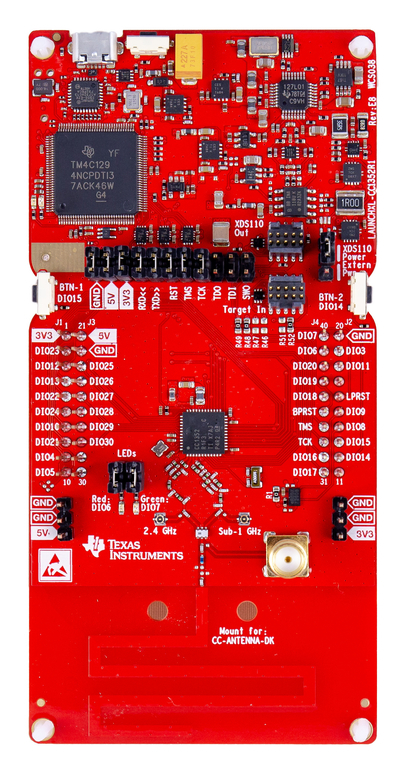
\includegraphics[width=0.5\textwidth]{./images/launchxl-cc1352r1.jpg}
		\caption{Placa \cite{placa}}
	\end{center}
\end{figure}

Aquesta placa permet el desenvolupament d'aplicacions en BLE utilitzant el microcontrolador CC1352 de Texas Instruments a continuació es descriuen les seves característiques principals \cite{placa_datasheet}.

El dispositiu CC1352R és multiprotocol i multibanda orientat a 2.4 GHz o sub-1GHz que serveix per a Thread, Zigbee, Bluetooth 5 Low Energy, IEEE 802.15.4g i 6LoWPAN. Pel que fa a memòria té 352 KB flash programable, 256 KB de ROM per a protocols i llibreries, 8 KB de Cache SRAM i 80 KB de RAM protegida amb paritat.
Pel que fa als perifèrics el més important és el ADC de 12 bits i 8 canals amb freqüència de mostreig de 200 Kmostres/s (multiplexat). També té Rellotge de Temps Real (RTC), acceleradors de operacions criptogràfiques i generador de números aleatoris.
La radio multibanda que té te un receptor amb sensibilitat de -121 dBm per a sub-1GHz i de -110 dBm a 50 Kbps o -105 dBm a 125 Kbps. El transmissor pot transmetre fins a 14 dBm sub-1GHz i 5dBm a 2.4 GHz.


\section{Software}
Per al desenvolupament de projectes per a la placa s'ha utilitzat el entorn de desenvolupament Code Composer Studio. El software és el SimpleLink(TM) CC13X2.
[Comentar tema versió]

\section{Project 0}
El Project 0 és el projecte instal·lat amb que les plaques vénen de fàbrica. Aquest projecte exposa certs serveis a través de BLE i et permet veure una comunicació simple entre la placa i un dispositiu mòbil.
La comunicació es fa a través del control dels dos LEDs que te la placa (els LEDs que estan directament controlats pel microcontrolador) i també per l'estat dels botons que hi ha a ambdós costats de la placa.
*Aquest projecte també inclou altres serveis en que no entrarem.

Aquest projecte serveix per tenir un bon exemple de com està dissenyada l'arquitectura dels serveis amb les seves característiques amb una relativa simple funcionalitat. A continuació s'analitzaran diferents parts dels atributs.

\subsection{Serveis de Butons i LEDs}

En la següent taula es poden veure tots els valors que hi ha tal i com estan en la taula d'atributs del servidor GATT.
Per facilitar la visualització de les dades s'han tret els zeros finals dels UUIDs propis però cal recordar que en total tenen 16 parells (128 bits en representació hexadecimal) i no només els 9 parells que surten a la taula.

\begin{center}
	\begin{table}[h!]
		\csvautotabular{data_files/projectzeroUUID.csv}
	\end{table}
\end{center}

Per poder entendre els atributs, al tenir UUID propis és necessari tenir en compte la documentació amb la que s'ha desenvolupat aquest projecte.

\begin{figure}[h!]
	\begin{center}
		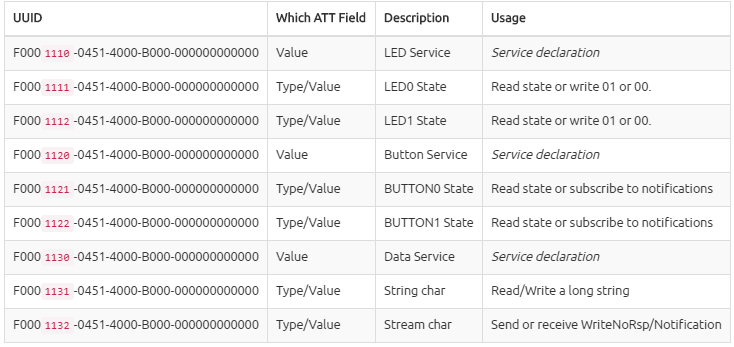
\includegraphics[width=\textwidth]{./images/Project_0_UUID.png}
		\caption{Definició dels UUIDs}
	\end{center}
\end{figure}

El primer que cal tenir clar és que en taula anterior (afegir link dinàmic) els valors estan representats amb l'ordre en que es reben i en general els serveis estandarditzats (i també aquest servei propi) utilitza \textit{little-endian} per enviar la informació.
Això resulta en que els caràcters hexadecimals queden (per parelles) ordenats al revés.

Al analitzar els atributs es pot veure com aquells que tenen el UUID 0x2800 en el seu valor només tenen un UUID corresponent al les definicions de serveis de LEDs i de botons.
Seguidament, als atribut amb UUID 0x2803 hi ha les definicions de les característiques, en el seu valor hi ha múltiples parts.
El primer parell hexadecimal correspon a les propietats. Just després hi ha dos parells hexadecimals que identifiquen el \textit{Handle} del atribut on hi ha la característica.
I per últim la resta de caràcters corresponen al UUID que identifica la característica.

\subsection{Propietats}
Les propietats d'accés són un valor que identifica quines operacions i procediments es poden fer sobre la característica.
El camp té 8 bits per defecte i cada un d'ells identifica una operació o procediment.
Es poden combinar qualsevol quantitat d'aquests bits per habilitar múltiples opcions.

\begin{center}
	\begin{tabular}{|c|c|l|}
		\hline
		Binary	&	Hex		&	Property	\\	\hline
		0000 0001	&	0x01	&	Broadcast\\	\hline
		0000 0010	&	0x02	&	Read	\\	\hline
		0000 0100	&	0x04	&	Write w/o Response	\\	\hline
		0000 1000	&	0x08	&	Write	\\	\hline
		0001 0000	&	0x10	&	Notification w/o ACK	\\	\hline
		0010 0000	&	0x20	&	Indication with ACK	\\	\hline
		0100 0000	&	0x40	&	Signed Writes	\\	\hline
		1000 0000	&	0x80	&	Aditional Properties	\\	\hline
	\end{tabular}
\end{center}

Primer de tot cal destacar la implementació de comunicacions amb o sense reconeixement. D'aquesta manera si preferim reduir la quantitat de missatges per estalviar bateria enlloc d'assegurar-se que s'ha rebut la informació es dona la opció.

Pel que fa les propietats en el Project 0 les característiques dels LEDs tenen el valor 0x0E que resulta en 0000 1110 per tant, es permet: llegir, escriure i escriure sense resposta.
En canvi les característiques del servei de botons té el valor 0x12 que suposa 0001 0010, per tant, es permet notificació sense reconeixement.

La notificació i indicació són funcions que ajuden a reduir el consum de recursos.
Quan volem saber en quin estat estan els botons de la placa contínuament es podria anar llegint el estat de la característica constantment però això suposarien molts missatges i reduiria el temps que els dispositius es poden adormir i així ser més eficients.
Per evitar aquest cas es pot configurar la característica tal que sigui la mateixa placa qui enviï el missatge automàticament quant el estat de la característica canviï.
D'aquesta manera el receptor només cal que escolti els missatges de la placa per tal de saber en quin estat està el botó.

En cas de que es vulgui indicació amb reconeixements és possible configurar-ho d'aquesta manera a través del atribut Configuració de Característica del Client identificat amb el UUID 0x2902 i estandarditzat en la especificació de Bluetooth.
Si el valor és 0 no hi ha transmissions, si el valor és 1 s'envien notificacions (sense reconeixement) i si el valor és 2 s'envien indicacions (notificacions amb reconeixement). 

El bit d'extensió de propietats, en cas que sigui 1 indica que existeix un atribut: Descriptor Propietats Esteses de Característica.
Aquest atribut te el UUID 0x2900 i el que permet és afegir més propietats de les que poden existir amb el espai limitat de 8 bits que hi ha per defecte.
Aquest sistema permet afegir fins a 16 bits més per indicar propietats, actualment estan els dos primers definits segons el estàndard i la resta estan reservats per a ús futur \cite{extended properties}.

Aquests 2 primers que estan definits són escriptura fiable i escriptura auxiliar.
L'escriptura fiable permet escriure valors amb un procediment diferent al habitual que permet assegurar-se que el valor que es vol modificar s'ha escrit i no hi han hagut errors.
Pel que fa  al'escriptura auxiliar permet escriptura al descriptor de característica [posar exemple].

\section{Experimentació}
Per comprendre millor com afecten els diferents paràmetres configurables corresponents a BLE i també les prestacions dels perifèrics de la placa es realitzaran els següents escenaris.

\subsection{ADC}
La placa té un convertidor analògic-digital que ens permetrà enviar senyals analògiques un cop s'han digitalitzat.


\subsection{Range}
\subsection{Throughput}
\cleardoublepage
\phantomsection
\chapter*{Conclusions}

Aquest projecte serveix per considerar si BLE és la tecnologia adequada per a les aplicacions de mesures mediambientals o biològiques.

%\section*{Taxa de dades necessària}

%Un dels dubtes a l'inici del treball era si aquesta tecnologia tenia una capacitat de transmissió suficient per a xarxes de sensors.
%Tot i que el Bluetooth Low Energy té bastant menys capacitat per transmetre dades comparant amb tecnologies com wifi, les dades necessàries en aquest tipus de xarxes acostumen a ser molt reduïdes.
%La tecnologia BLE no és capaç de transmetre vídeo o àudio en temps real però és suficient per transmetre fluxos de dades de sensors amb mesures biològiques o mediambientals.

\section*{Abast}

Com s'ha comentat, l'abast de la tecnologia BLE ve limitat tant per la distància entre transmissor i receptor com per les interferències.
En mesures biològiques es pot considerar que el transmissor i el receptor estaran relativament a prop, per tant, no hi haurà problemes d'abast.
En canvi, per a mesures ambientals si considerem instal·lacions privades en habitatges, cal tenir en compte els obstacles que s'oposen al senyal.
També cal considerar la interferència més que probable de les tecnologies amb les quals BLE comparteix espectre com wifi, altres dispositius intel·ligents o amb Bluetooth Clàssic mateix.
Per combatre aquests desavantatges BLE té múltiples estratègies.
Primerament, sempre és possible augmentar la potència de transmissió (fins al límit permès), però reduint el cicle de vida de la bateria.
També es poden utilitzar capes físiques que implementen més redundància (\textit{LE Coded}).
Finalment, BLE implementa salts en freqüència i la \textit{Slot Availability Mask} per combatre interferències.

Totes aquestes tècniques augmenten la complexitat del protocol però ajuden a poder tenir un gran abast.
A més a més, BLE utilitza canals de freqüència estrets comparats amb altres tecnologies com wifi per tant, les interferències afecten menys a BLE que a altres tecnologies amb canals més amples.

\section*{Consum d'Energia}

BLE és dels protocols que permet consumir menys energia per a transmetre informació.
Això només serà un avantatge quan els sensors estiguin alimentats per bateria i la transmissió sigui el que consumeix més energia de tot el sistema.
Si els sensors tenen pantalles, s'alimenten de la instal·lació elèctrica, fan un processament de les dades o emmagatzemen les dades localment; és possible que el consum de la transmissió no sigui significant.
En aquests casos no s'ha d'escollir el protocol de transmissió segons el consum, ja que el temps entre recàrregues no es veu especialment afectat pel protocol.

En els escenaris on és important tenir un consum baix d'energia, el protocol BLE és una molt bona opció.
Com ja s'ha comentat múltiples vegades, BLE defineix moltes opcions d'implementació i això suposa una flexibilitat molt important.
Aquesta flexibilitat permet, per exemple, poder prescindir de les transmissions redundants com el reconeixement.
Tanmateix, es pot utilitzar la latència d'esclau per reduir els esdeveniments d'una connexió quan no són necessaris.
També, permet transmetre molta informació sense necessitat d'establir una connexió.

Així doncs, poder evitar realitzar tots aquests procediments permet reduir significativament el consum que suposa la transmissió de dades i fa possible augmentar el cicle de vida de la bateria o reduir la mida d'aquesta.
Gràcies a BLE és possible que dispositius no hagin d'estar connectats a cap altre dispositiu a través de cables ni a la xarxa elèctrica.

\section*{Penetració del mercat}

Quan en un projecte hi ha usuaris involucrats d'alguna manera, és molt probable que el telèfon mòbil sigui un component important.
BLE té el gran avantatge que ve incorporat en tots els mòbils intel·ligents.
Això facilita l'ús, ja que els usuaris estan més acostumats, i simplifica l'arquitectura d'un desplegament.
L'arquitectura és més simple perquè el mateix dispositiu mòbil és el receptor de les dades.
En cas de no utilitzar BLE, no hi ha cap tecnologia de baix consum que es pugui connectar directament amb els telèfons dels usuaris.
Altres tecnologies acostumen a utilitzar un dispositiu entre els sensors i els usuaris que s'anomena concentrador o \textit{hub}.
A l'afegir un nou dispositiu s'incrementa el cost d'un desplegament.
A més a més, augmenta la complexitat del flux de dades i també incrementa l'ús de la banda freqüencial, ja que calen més transmissions per la mateixa quantitat d'informació.

En canvi, en el cas de connexió directa fins al terminal de l'usuari BLE és perfecte.
No només està present en telèfons mòbils sinó també en: joguines, televisors, electrodomèstics, càmeres, comandaments a distància, entre d'altres...
En total es preveu la producció de 7.500 milions de dispositius entre 2020 i 2024 amb un creixement del 26\% anual segons el SIG \cite{Bluetooth_Market_Update_2020}.


%%%  BIBLIOGRAFIA
%%%%%%%%%%%%%%%%%%%%%%%%%%%%%%%%%%%%%%%%%%%%%%%%%%%%%%%%%%%%%%%%%%%%%%%%%%

%%% Per la bibliografia hi ha 2 opcions: generarla amb la utilitat BibTeX 
%%%                                      o fer-la ''a ma''
%%% NOTA: podeu trobar facilment informació sobre BibTeX a:
%%%  http://www.ctan.org/tex-archive/biblio/bibtex/contrib/doc/

%%% OPCIO 1: BibTeX (recomanat) -> descomentar les comandes seguents:
%\bibliographystyle{unsrt}   %% Estil de bibliografia EETAC
%\cleardoublepage
%\phantomsection
% Indicar aqui el(s) fitxer(s) que contenen la bibliografia
%\bibliography{fitxer1,...,fitxerN}  
%\pdfbookmark{Bibliografia}{sec:biblio}

%%% OPCIO 2: bibliografia manual
%%%
%%% L'argument d'entrada es el numero de referencies que s'inclouen
\cleardoublepage
\phantomsection
\begin{thebibliography}{2}

%% Llibres:  Autor/s (cognoms i inicials dels noms), títol del llibre (en cursiva), editor, ciutat i any de publicació. Quan es cita el capítol d'un llibre s'ha d'indicar el títol del capítol (entre cometes), el títol del llibre (en cursiva) i els números de pàgines amb la primera i la darrera incloses.

\bibitem{Bluetooth Specification}
Bluetooth Special Interest Group
``Bluetooth Core Specification``
(Revision 5.2)

%%  Exemple de capitol en llibre
\bibitem{prova1} 
Cognoms-autor, Inicial-nom.
``Títol del capítol''. {\it Títol del llibre}.
(Editor. Ciutat. Any publicació): pagina1--paginaN.

%%  Exemple de d'article en revista
\bibitem{prova2} 
Cognoms-autor, Inicial-nom.
``Títol de l'article''. {\it Títol de la revista}.
{\bf volum}(numero),
pagina1--paginaN. (Any publicació) 

\end{thebibliography}

%%%%%%%%%%%%%%%%%%%%%%%%%%%%%%%%%%%%%%%%%%%%%%%%%%%%%%%%%%%%%%%%%%%%%%%%%%
%%%%%%                           APENDIXS                         %%%%%%%%
%%%%%%%%%%%%%%%%%%%%%%%%%%%%%%%%%%%%%%%%%%%%%%%%%%%%%%%%%%%%%%%%%%%%%%%%%%
\pagestyle{empty}  % no tocar

%% Descomentar una de les dues línies següents, en funció de:
%%  a) els apendixs s'encuadernaran apart (amb portada) 
%%  b) els apendixs s'enquadernen amb el mateix projecte (sense portada). 
%% Recordeu que si tot el document (amb apèndixs) excedeix les 100 pagines 
%% s'ha d'enquadernar a part
%\appendix\ambportada
\appendix\senseportada


%%%%%%%%%%%%%%%%%%%%%%%%%%%%%%%%%%%%%%%%%%%%%%%%%%%%%%%%%%%%%%%%%%%%%%%%%%
%%%%%% INCLOURE A PARTIR D'AQUI TOTS ELS CAPÍTOLS DELS APENDIXS   %%%%%%%%
%%%%%%%%%%%%%%%%%%%%%%%%%%%%%%%%%%%%%%%%%%%%%%%%%%%%%%%%%%%%%%%%%%%%%%%%%%




\chapter{Taula de atributs del Project 0}

\begin{table}[h!]
	\begin{center}
		\tiny
		\csvautotabular{data_files/projectzeroUUID.csv}
	\end{center}
\end{table}




%%%%%%%%%%%%%%%%%%%%%%%%%%%%%%%%%%%%%%%%%%%%%%%%%%%%%%%%%%%%%%%%%%%%%%%%%%
%%%%%%%%%%%%%%%%%%%%%%%%%%%%%%%%%%%%%%%%%%%%%%%%%%%%%%%%%%%%%%%%%%%%%%%%%%
%%%%%%%%%%%%%%%%%%%%%%%%%%%%%%%%%%%%%%%%%%%%%%%%%%%%%%%%%%%%%%%%%%%%%%%%%%
% i  aixo es tot! ;)
\end{document}






